% A LaTeX template for MSc Thesis submissions to 
% Politecnico di Milano (PoliMi) - School of Industrial and Information Engineering
%
% S. Bonetti, A. Gruttadauria, G. Mescolini, A. Zingaro
% e-mail: template-tesi-ingind@polimi.it
%
% Last Revision: October 2021
%
% Copyright 2021 Politecnico di Milano, Italy. NC-BY

\documentclass{Configuration_Files/PoliMi3i_thesis}

%------------------------------------------------------------------------------
%	REQUIRED PACKAGES AND  CONFIGURATIONS
%------------------------------------------------------------------------------

% CONFIGURATIONS
\usepackage{parskip} % For paragraph layout
\usepackage{setspace} % For using single or double spacing
\usepackage{emptypage} % To insert empty pages
\usepackage{multicol} % To write in multiple columns (executive summary)
\setlength\columnsep{15pt} % Column separation in executive summary
\setlength\parindent{0pt} % Indentation
\raggedbottom  

% PACKAGES FOR TITLES
\usepackage{titlesec}
% \titlespacing{\section}{left spacing}{before spacing}{after spacing}
\titlespacing{\section}{0pt}{3.3ex}{2ex}
\titlespacing{\subsection}{0pt}{3.3ex}{1.65ex}
\titlespacing{\subsubsection}{0pt}{3.3ex}{1ex}
\usepackage{color}

% PACKAGES FOR LANGUAGE AND FONT
\usepackage[english]{babel} % The document is in English  
\usepackage[utf8]{inputenc} % UTF8 encoding
\usepackage[T1]{fontenc} % Font encoding
\usepackage[11pt]{moresize} % Big fonts

% PACKAGES FOR IMAGES
\usepackage{graphicx}
\usepackage{transparent} % Enables transparent images
\usepackage{eso-pic} % For the background picture on the title page
\usepackage{subfig} % Numbered and caption subfigures using \subfloat.
\usepackage{tikz} % A package for high-quality hand-made figures.
\usetikzlibrary{}
\graphicspath{{./Images/}} % Directory of the images
\usepackage{caption} % Coloured captions
\usepackage{xcolor} % Coloured captions
\usepackage{amsthm,thmtools,xcolor} % Coloured "Theorem"
\usepackage{float}

% STANDARD MATH PACKAGES
\usepackage{amsmath}
\usepackage{amsthm}
\usepackage{amssymb}
\usepackage{amsfonts}
\usepackage{bm}
\usepackage[overload]{empheq} % For braced-style systems of equations.
\usepackage{fix-cm} % To override original LaTeX restrictions on sizes

% PACKAGES FOR TABLES
\usepackage{tabularx}
\usepackage{longtable} % Tables that can span several pages
\usepackage{colortbl}

% PACKAGES FOR ALGORITHMS (PSEUDO-CODE)
\usepackage{algorithm}
\usepackage{algorithmic}

% PACKAGES FOR REFERENCES & BIBLIOGRAPHY
\usepackage[colorlinks=true,linkcolor=black,anchorcolor=black,citecolor=black,filecolor=black,menucolor=black,runcolor=black,urlcolor=black]{hyperref} % Adds clickable links at references
\usepackage{cleveref}
% I CHANGED BELOW TWO LINES
\bibliographystyle{unsrtnat}
\usepackage[numbers,sort&compress]{natbib}

% OTHER PACKAGES
\usepackage{pdfpages} % To include a pdf file
\usepackage{afterpage}
\usepackage{lipsum} % DUMMY PACKAGE
\usepackage{fancyhdr} % For the headers
\fancyhf{}

% Input of configuration file. Do not change config.tex file unless you really know what you are doing. 
% Define blue color typical of polimi
\definecolor{bluepoli}{cmyk}{0.4,0.1,0,0.4}

% Custom theorem environments
\declaretheoremstyle[
  headfont=\color{bluepoli}\normalfont\bfseries,
  bodyfont=\color{black}\normalfont\itshape,
]{colored}

% Set-up caption colors
\captionsetup[figure]{labelfont={color=bluepoli}} % Set colour of the captions
\captionsetup[table]{labelfont={color=bluepoli}} % Set colour of the captions
\captionsetup[algorithm]{labelfont={color=bluepoli}} % Set colour of the captions

\theoremstyle{colored}
\newtheorem{theorem}{Theorem}[chapter]
\newtheorem{proposition}{Proposition}[chapter]

% Enhances the features of the standard "table" and "tabular" environments.
\newcommand\T{\rule{0pt}{2.6ex}}
\newcommand\B{\rule[-1.2ex]{0pt}{0pt}}

% Pseudo-code algorithm descriptions.
\newcounter{algsubstate}
\renewcommand{\thealgsubstate}{\alph{algsubstate}}
\newenvironment{algsubstates}
  {\setcounter{algsubstate}{0}%
   \renewcommand{\STATE}{%
     \stepcounter{algsubstate}%
     \Statex {\small\thealgsubstate:}\space}}
  {}

% New font size
\newcommand\numfontsize{\@setfontsize\Huge{200}{60}}

% Title format: chapter
\titleformat{\chapter}[hang]{
\fontsize{50}{20}\selectfont\bfseries\filright}{\textcolor{bluepoli} \thechapter\hsp\hspace{2mm}\textcolor{bluepoli}{|   }\hsp}{0pt}{\huge\bfseries \textcolor{bluepoli}
}

% Title format: section
\titleformat{\section}
{\color{bluepoli}\normalfont\Large\bfseries}
{\color{bluepoli}\thesection.}{1em}{}

% Title format: subsection
\titleformat{\subsection}
{\color{bluepoli}\normalfont\large\bfseries}
{\color{bluepoli}\thesubsection.}{1em}{}

% Title format: subsubsection
\titleformat{\subsubsection}
{\color{bluepoli}\normalfont\large\bfseries}
{\color{bluepoli}\thesubsubsection.}{1em}{}

% Shortening for setting no horizontal-spacing
\newcommand{\hsp}{\hspace{0pt}}

\makeatletter
% Renewcommand: cleardoublepage including the background pic
\renewcommand*\cleardoublepage{%
  \clearpage\if@twoside\ifodd\c@page\else
  \null
  \AddToShipoutPicture*{\BackgroundPic}
  \thispagestyle{empty}%
  \newpage
  \if@twocolumn\hbox{}\newpage\fi\fi\fi}
\makeatother

%For correctly numbering algorithms
\numberwithin{algorithm}{chapter}

%----------------------------------------------------------------------------
%	NEW COMMANDS DEFINED
%----------------------------------------------------------------------------

% EXAMPLES OF NEW COMMANDS
\newcommand{\bea}{\begin{eqnarray}} % Shortcut for equation arrays
\newcommand{\eea}{\end{eqnarray}}
\newcommand{\e}[1]{\times 10^{#1}}  % Powers of 10 notation

%----------------------------------------------------------------------------
%	ADD YOUR PACKAGES (be careful of package interaction)
%----------------------------------------------------------------------------

%----------------------------------------------------------------------------
%	ADD YOUR DEFINITIONS AND COMMANDS (be careful of existing commands)
%----------------------------------------------------------------------------

%----------------------------------------------------------------------------
%	BEGIN OF YOUR DOCUMENT
%----------------------------------------------------------------------------

\begin{document}

\fancypagestyle{plain}{%
\fancyhf{} % Clear all header and footer fields
\fancyhead[RO,RE]{\thepage} %RO=right odd, RE=right even
\renewcommand{\headrulewidth}{0pt}
\renewcommand{\footrulewidth}{0pt}}

%----------------------------------------------------------------------------
%	TITLE PAGE
%----------------------------------------------------------------------------

\pagestyle{empty} % No page numbers
\frontmatter % Use roman page numbering style (i, ii, iii, iv...) for the preamble pages

\puttitle{
	title=Title Related to Microservices, % Title of the thesis
	name=Ömer Esas, % Author Name and Surname
	course=Computer Science and Engineering - Ingegneria Informatica, % Study Programme (in Italian)
	ID  = 917254,  % Student ID number (numero di matricola)
	advisor= Prof. Elisabetta Di Nitto, % Supervisor name
	coadvisor={Name Surname, Name Surname}, % Co-Supervisor name, remove this line if there is none
	academicyear={2021-22},  % Academic Year
} % These info will be put into your Title page 

%----------------------------------------------------------------------------
%	PREAMBLE PAGES: ABSTRACT (inglese e italiano), EXECUTIVE SUMMARY
%----------------------------------------------------------------------------
\startpreamble
\setcounter{page}{1} % Set page counter to 1

% ABSTRACT IN ENGLISH
\chapter*{Abstract} 
Here goes the Abstract in English of your thesis followed by a list of keywords.
\\
\\
\textbf{Keywords:} here, the keywords, of your thesis % Keywords

% ABSTRACT IN ITALIAN
\chapter*{Abstract in lingua italiana}
Qui va l'Abstract in lingua italiana della tesi seguito dalla lista di parole chiave.
\\
\\
\textbf{Parole chiave:} qui, vanno, le parole chiave, della tesi % Keywords (italian)

%----------------------------------------------------------------------------
%	LIST OF CONTENTS/FIGURES/TABLES/SYMBOLS
%----------------------------------------------------------------------------

% TABLE OF CONTENTS
\thispagestyle{empty}
\tableofcontents % Table of contents 
\thispagestyle{empty}
\cleardoublepage

%-------------------------------------------------------------------------
%	THESIS MAIN TEXT
%-------------------------------------------------------------------------
% In the main text of your thesis you can write the chapters in two different ways:
%
%(1) As presented in this template you can write:
%    \chapter{Title of the chapter}
%    *body of the chapter*
%
%(2) You can write your chapter in a separated .tex file and then include it in the main file with the following command:
%    \chapter{Title of the chapter}
%    \input{chapter_file.tex}
%
% Especially for long thesis, we recommend you the second option.

\addtocontents{toc}{\vspace{2em}} % Add a gap in the Contents, for aesthetics
\mainmatter % Begin numeric (1,2,3...) page numbering

% --------------------------------------------------------------------------
% NUMBERED CHAPTERS % Regular chapters following
% --------------------------------------------------------------------------
\chapter{Introduction}

\chapter{State of the Art}
\label{ch:art}%

\section{Microservice Architecture}
\label{sec:ms_arch}

Although the microservice architecture style has already been a de-facto standard for some large tech companies, and is being embraced by numerous firms in the industry, because of the novelty of the architecture, not all developers and architects in the tech industry and researchers in the academia are aware of what it means and which paradigms it advertises.
Microservice architecture is, not in the least meaning of the word, vastly different from the traditional way of building a web application, namely the monolithic architecture.
Hence, it is a valuable effort to define microservice architecture, what it is about and describe features and trends from which this rather unorthodox architecture emerged.
\\
Most importantly, microservice architecture is, as the name suggests, a software architecture.
There are numerous and slightly different definitions based on the particular discipline of software engineering for what a software architecture is.
However, a very simple yet powerful definition is, a (software) architecture is a representation of significant design decisions that shape a system, where significant is measured by the cost of change \cite{booch}. 
In the case for microservice architecture, the most signification design decision is, splitting the system into small, autonomous services that work together.
Focusing on each element of this design decision will bring about more clarity about the architecture.
\\
First, the microservice architecture divide the system into parts, as other architectural styles do, based on various point of views of the system.
Single Responsibility Principle, one of the famous SOLID principles of software engineering, promotes the idea that every module, class or a function in a computer program should have responsibility over a single part of that program's functionality, and it should encapsulate that part \cite{srp}.
The microservice architecture takes that idea to the extreme and encourages developing independent microservices that tackles just one business functionality.
Unlike a monolithic application, the system is not layered as database, back-end and front-end, or more generally, data, logic and UX layers, but consists of microservices that are created around business capabilities, as displayed in Figure~\ref{fig:monovsmicro}.

\begin{figure}[H]
    \centering
    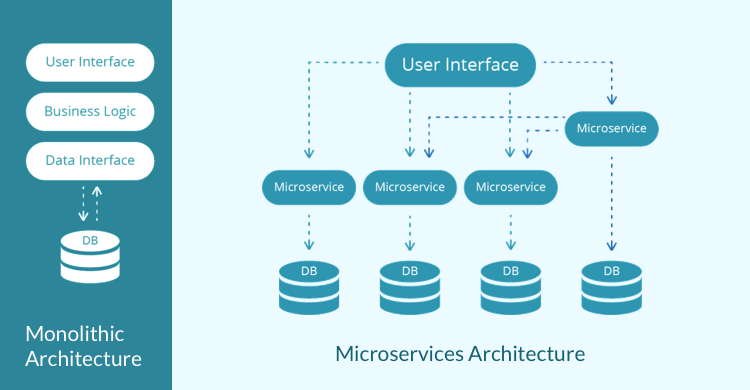
\includegraphics[width=0.75\textwidth]{myImages/monolithic-vs-microservices.png}
    \caption{Monolithic vs Microservice Architecture}
    \label{fig:monovsmicro}
\end{figure}

Second, the microservice architecture advocates for those services to be small.
It is not easy and in some cases inaccurate (e.g, in terms of LOC) to give an estimate of the magnitude of a service, however, a rule of thumb to keep in mind is, microservices should be small enough and not smaller \cite{newman}.
Each service should focus on one business functionality and do it well.
\\
Third, and the last major aspect that defines the microservice architecture is autonomy.
Each service in the microservice architecture is a separate entity, even to the degree that they are mostly designed, developed and deployed by separate teams.
Each team has staff that can together carry out full range of skills required for development, such as database, UX and project management.
\\
At this point, in order to summarize the mentioned major aspects of the microservice architecture and make the architecture more concrete by adding a bit more detail about the implementation, it is a good opportunity to take a look at the definition of the microservice architecture given by an influential software engineer in the field.
According to M. Fowler, the microservice architecture is, "in short, an approach to developing a single application as a suite of small services, each running in its own process and communicating with lightweight mechanisms, often an HTTP resource API.
These services are built around business capabilities and independently deployable by fully automated deployment machinery.
There is a bare minimum of centralized management of these services, which may be written in different programming languages and use different data storage technologies." \cite{microdef}.
In the next section, each characteristic of the microservice architecture is explained in more detail.

\subsection{General Characteristics}
\label{subsec:chars}

\begin{itemize}
    \item Each microservice is developed by a small, cross-functional team.
    The team decides which programming language(s) and technology stack to choose to implement the microservice, and has their own CI/CD tools for testing, release and deployment.
    Each microservice is considered not just a project, but a product, and the development teams are responsible also for the deployment and production process of their microservice, in the Amazon's notion of "you build it, you run it" \cite{youbuild}.
    
    \item Each microservice is a light-weight component that is independently deployable. In case of a change in a particular library, systems that have multiple libraries in a single process like a monolithic architecture has to redeploy entire application. Instead, in a same scenario, having multiple services facilitates redeploying only the changed service. Moreover, this kind of ease in deployment enables the system to be more fault-tolerant and scalable in a more dynamic way, as illustrated Figure~\ref{fig:scalability}.
    
    \begin{figure}[H]
    \centering
    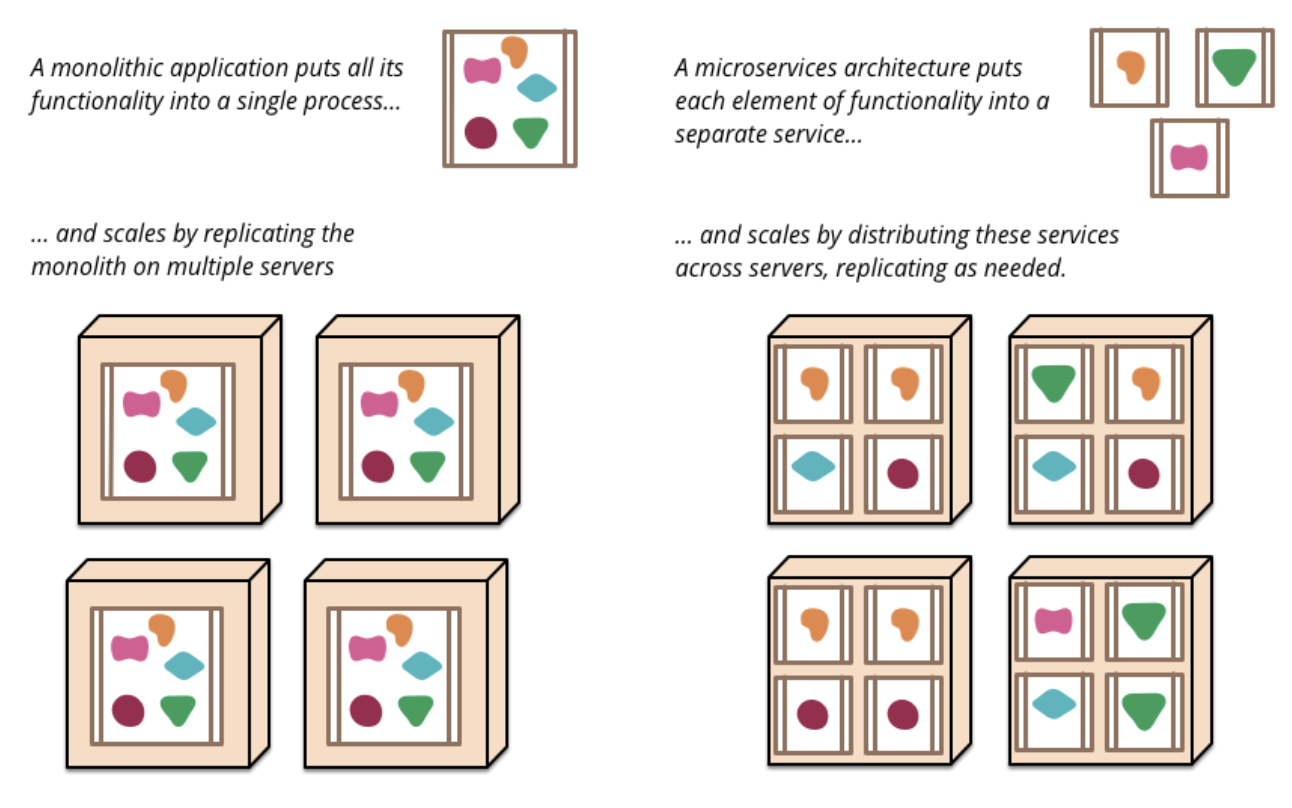
\includegraphics[width=0.75\textwidth]{myImages/scalable.png}
    \caption{Scalability in Monolithic vs Microservice Apps}
    \label{fig:scalability}
\end{figure}

    \item Microservices communicate with each other by means of network calls, using well-defined APIs, and simple protocols like REST over HTTP. While some other architectures incorporate smart (and heavy-weight) messaging mechanisms, such as Enterprise Service Buses (ESB) that can do routing, transformation, choreography and some business logic, the microservice architecture opt for simple communication infrastructure that can do basic routing of messages. In short, they have smart endpoints and dumb pipes.

    \item Each microservice is a loosely-coupled business unit, that is responsible for a single part of the business capability.
    Each model of a microservice is designed on a Bounded Context, which is a part of Domain Driven Design technique \cite{boundedcontext}. Conceptual model of the real world entities are decentralized, meaning that the representation (name) and modeling (attributes) of same real world entities are distinct. Figure~\ref{fig:micromodel} illustrates an example bounded context design and highlights the different representation of the same entity in different microservices.
    
    \begin{figure}[H]
    \centering
    \subfloat[Same Concept as Different Model Entities in Different Microservices\label{fig:micromodel1}]{
        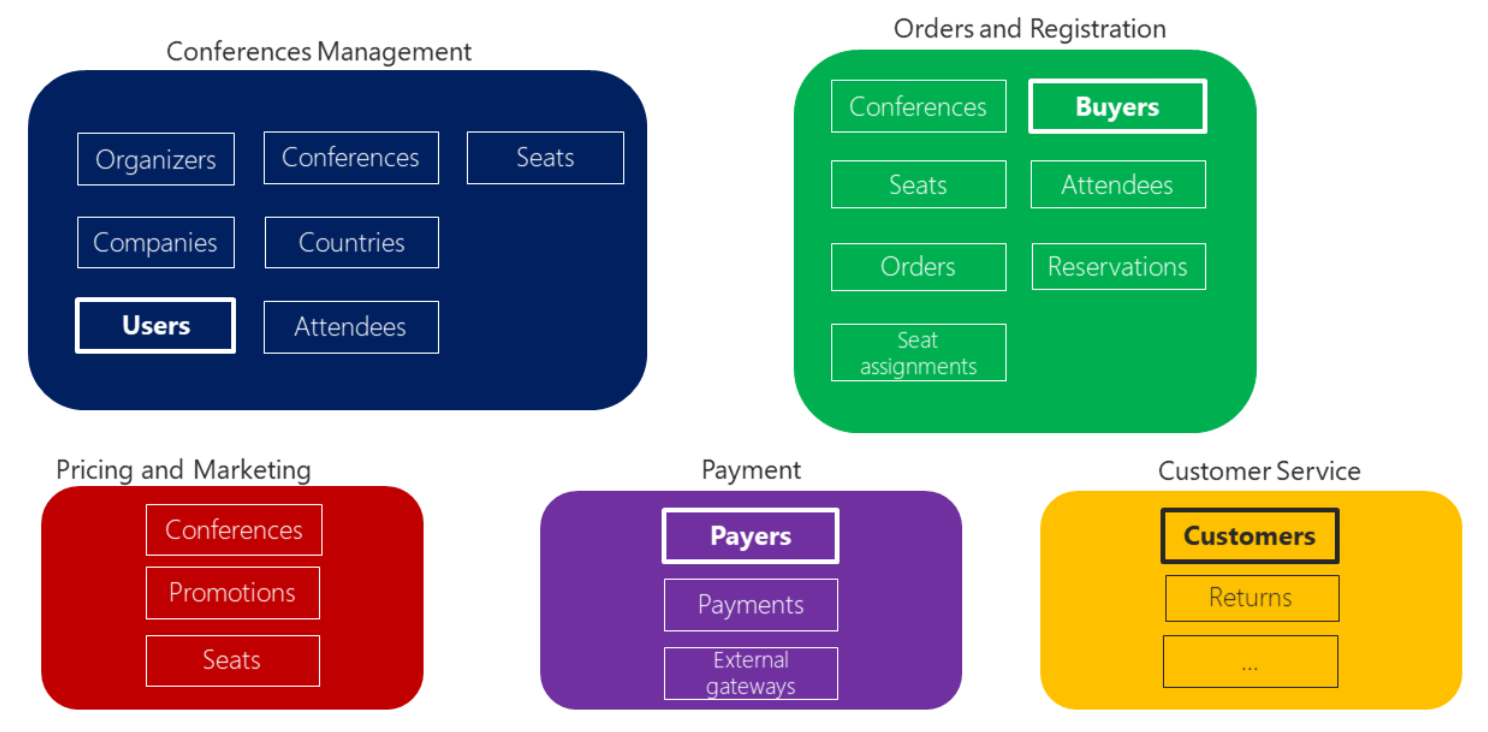
\includegraphics[scale=0.4]{myImages/micromodel1.png}
    }
    \quad
    \subfloat[Decomposing Traditional Data Models\label{fig:micromodel2}]{
        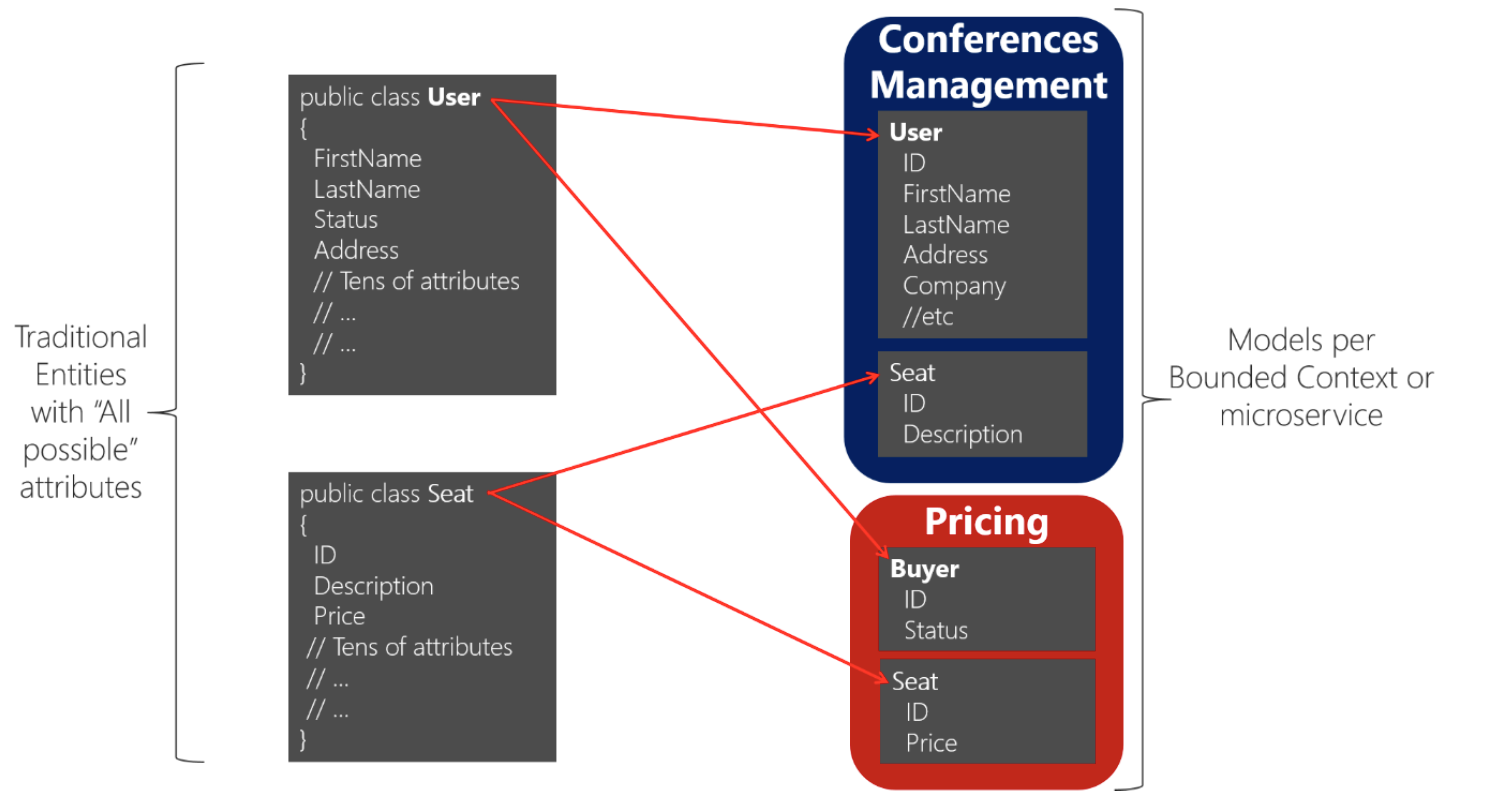
\includegraphics[scale=0.45]{myImages/micromodel2.png}
    }
    \caption{A Microservices Design Using Bound Context Model per Microservice}
    \label{fig:micromodel}
\end{figure}

    \item Just like the decentralized modeling, the persistence layer of the whole application is decentralized, in other words, each microservice and associated team is responsible for managing their own data. The team decides on which kind of database (SQL, NoSQL, graph, columnar, etc) they make use of, taking into consideration their own models and needs.

\end{itemize}

\subsection{Differences with Service Oriented Architecture}
\label{subsec:diff}

\section{Design Patterns and Anti-Patterns in Microservices}
\label{sec:patterns}

\subsection{Design Patterns}
\label{subsec:designpattern}

\subsection{Anti-Patterns}
\label{subsec:antipattern}

\chapter{Adopted Methodology}
\label{ch:method}%

\section{Classification of Patterns}
\label{sec:class_method}

\section{Selection of Open Source Projects}
\label{sec:select_method}

\section{Detection of Patterns}
\label{sec:detection_method}

\chapter{Results}
\label{ch:results}%

\section{Resulting Classification of Patterns}
\label{sec:class_result}

\section{Selected Open Source Projects}
\label{sec:select_result}

\section{Detected Patterns in Selected Projects}
\label{sec:detection_result}

\section{Discussion of Findings}
\label{sec:discussion}

\chapter{Conclusion}
\label{ch:conclusion}%

%-------------------------------------------------------------------------
%	BIBLIOGRAPHY
%-------------------------------------------------------------------------

\addtocontents{toc}{\vspace{2em}} % Add a gap in the Contents, for aesthetics
\bibliography{myThesisBib}

%-------------------------------------------------------------------------
%	APPENDICES
%-------------------------------------------------------------------------

\cleardoublepage
\addtocontents{toc}{\vspace{2em}} % Add a gap in the Contents, for aesthetics
\appendix
\chapter{Appendix A}
If you need to include an appendix to support the research in your thesis, you can place it at the end of the manuscript.
An appendix contains supplementary material (figures, tables, data, codes, mathematical proofs, surveys, \dots)
which supplement the main results contained in the previous chapters.

% LIST OF FIGURES
\listoffigures

% LIST OF TABLES
\listoftables

% LIST OF ABBREVIATIONS
% Write out the List of Symbols in this page
\chapter*{List of Abbreviations}
\begin{table}[H]
    \centering
    \begin{tabular}{ll}
        \textbf{Abbreviation} & \textbf{Description} \\\hline\\[-9px]
        UX & User Experience \\[2px]
        LOC & Lines of Code \\[2px]
        HTTP & Hypertext Transfer Protocol \\[2px]
        API & Application Programming Interface \\[2px]
        CI/CD & Continuous Integration / Continuous Delivery \\[2px]
        SQL & Structured Query Language \\[2px]
        NoSQL & Not-Only-SQL, to refer to different kinds of non-relational databases \\[2px]
        REST & Representational State Transfer \\[2px]
        ESB & Enterprise Service Bus \\[2px]
        BC & Bounded Context \\[2px]
        DDD & Domain Driven Design \\[2px]
    \end{tabular}
\end{table}

% ACKNOWLEDGEMENTS
\chapter*{Acknowledgements}
Here you might want to acknowledge someone.

\cleardoublepage

\end{document}
